%  LaTeX support: latex@mdpi.com
%  In case you need support, please attach all files that are necessary for compiling as well as the log file, and specify the details of your LaTeX setup (which operating system and LaTeX version / tools you are using).

%=================================================================
\documentclass[water,article,submit,moreauthors,pdftex]{mdpi}

% If you would like to post an early version of this manuscript as a preprint, you may use preprint as the journal and change 'submit' to 'accept'. The document class line would be, e.g., \documentclass[preprints,article,accept,moreauthors,pdftex]{mdpi}. This is especially recommended for submission to arXiv, where line numbers should be removed before posting. For preprints.org, the editorial staff will make this change immediately prior to posting.

%% Some pieces required from the pandoc template
\setlist[itemize]{leftmargin=*,labelsep=5.8mm}
\setlist[enumerate]{leftmargin=*,labelsep=4.9mm}


%--------------------
% Class Options:
%--------------------
%----------
% journal
%----------
% Choose between the following MDPI journals:
% acoustics, actuators, addictions, admsci, aerospace, agriculture, agriengineering, agronomy, algorithms, animals, antibiotics, antibodies, antioxidants, applsci, arts, asc, asi, atmosphere, atoms, axioms, batteries, bdcc, behavsci , beverages, bioengineering, biology, biomedicines, biomimetics, biomolecules, biosensors, brainsci , buildings, cancers, carbon , catalysts, cells, ceramics, challenges, chemengineering, chemistry, chemosensors, children, cleantechnol, climate, clockssleep, cmd, coatings, colloids, computation, computers, condensedmatter, cosmetics, cryptography, crystals, dairy, data, dentistry, designs , diagnostics, diseases, diversity, drones, econometrics, economies, education, electrochem, electronics, energies, entropy, environments, epigenomes, est, fermentation, fibers, fire, fishes, fluids, foods, forecasting, forests, fractalfract, futureinternet, futurephys, galaxies, games, gastrointestdisord, gels, genealogy, genes, geohazards, geosciences, geriatrics, hazardousmatters, healthcare, heritage, highthroughput, horticulturae, humanities, hydrology, ijerph, ijfs, ijgi, ijms, ijns, ijtpp, informatics, information, infrastructures, inorganics, insects, instruments, inventions, iot, j, jcdd, jcm, jcp, jcs, jdb, jfb, jfmk, jimaging, jintelligence, jlpea, jmmp, jmse, jnt, jof, joitmc, jpm, jrfm, jsan, land, languages, laws, life, literature, logistics, lubricants, machines, magnetochemistry, make, marinedrugs, materials, mathematics, mca, medicina, medicines, medsci, membranes, metabolites, metals, microarrays, micromachines, microorganisms, minerals, modelling, molbank, molecules, mps, mti, nanomaterials, ncrna, neuroglia, nitrogen, notspecified, nutrients, ohbm, particles, pathogens, pharmaceuticals, pharmaceutics, pharmacy, philosophies, photonics, physics, plants, plasma, polymers, polysaccharides, preprints , proceedings, processes, proteomes, psych, publications, quantumrep, quaternary, qubs, reactions, recycling, religions, remotesensing, reports, resources, risks, robotics, safety, sci, scipharm, sensors, separations, sexes, signals, sinusitis, smartcities, sna, societies, socsci, soilsystems, sports, standards, stats, surfaces, surgeries, sustainability, symmetry, systems, technologies, test, toxics, toxins, tropicalmed, universe, urbansci, vaccines, vehicles, vetsci, vibration, viruses, vision, water, wem, wevj

%---------
% article
%---------
% The default type of manuscript is "article", but can be replaced by:
% abstract, addendum, article, benchmark, book, bookreview, briefreport, casereport, changes, comment, commentary, communication, conceptpaper, conferenceproceedings, correction, conferencereport, expressionofconcern, extendedabstract, meetingreport, creative, datadescriptor, discussion, editorial, essay, erratum, hypothesis, interestingimages, letter, meetingreport, newbookreceived, obituary, opinion, projectreport, reply, retraction, review, perspective, protocol, shortnote, supfile, technicalnote, viewpoint
% supfile = supplementary materials

%----------
% submit
%----------
% The class option "submit" will be changed to "accept" by the Editorial Office when the paper is accepted. This will only make changes to the frontpage (e.g., the logo of the journal will get visible), the headings, and the copyright information. Also, line numbering will be removed. Journal info and pagination for accepted papers will also be assigned by the Editorial Office.

%------------------
% moreauthors
%------------------
% If there is only one author the class option oneauthor should be used. Otherwise use the class option moreauthors.

%---------
% pdftex
%---------
% The option pdftex is for use with pdfLaTeX. If eps figures are used, remove the option pdftex and use LaTeX and dvi2pdf.

%=================================================================
\firstpage{1}
\makeatletter
\setcounter{page}{\@firstpage}
\makeatother
\pubvolume{xx}
\issuenum{1}
\articlenumber{5}
\pubyear{2019}
\copyrightyear{2019}
%\externaleditor{Academic Editor: name}
\history{Received: date; Accepted: date; Published: date}
\updates{yes} % If there is an update available, un-comment this line

%% MDPI internal command: uncomment if new journal that already uses continuous page numbers
%\continuouspages{yes}

%------------------------------------------------------------------
% The following line should be uncommented if the LaTeX file is uploaded to arXiv.org
%\pdfoutput=1

%=================================================================
% Add packages and commands here. The following packages are loaded in our class file: fontenc, calc, indentfirst, fancyhdr, graphicx, lastpage, ifthen, lineno, float, amsmath, setspace, enumitem, mathpazo, booktabs, titlesec, etoolbox, amsthm, hyphenat, natbib, hyperref, footmisc, geometry, caption, url, mdframed, tabto, soul, multirow, microtype, tikz

%=================================================================
%% Please use the following mathematics environments: Theorem, Lemma, Corollary, Proposition, Characterization, Property, Problem, Example, ExamplesandDefinitions, Hypothesis, Remark, Definition
%% For proofs, please use the proof environment (the amsthm package is loaded by the MDPI class).

%=================================================================
% Full title of the paper (Capitalized)
\Title{Does the COMPAS Needle Always Point Towards Equity? Finding
Fairness in the COMPAS Risk Assessment Algorithm: A Case Study}

% Authors, for the paper (add full first names)
\Author{Amrita Acharya$^{1}$, Dianne Caravela$^{1}$, Eunice
Kim$^{1}$, Emma Kornberg$^{1}$, Elisabeth Nesmith$^{1}$}

% Authors, for metadata in PDF
\AuthorNames{Amrita Acharya, Dianne Caravela, Eunice Kim, Emma
Kornberg, Elisabeth Nesmith}

% Affiliations / Addresses (Add [1] after \address if there is only one affiliation.)
\address{%
$^{1}$ \quad Statistical and Data Sciences Smith College Northampton, MA
01063; \href{mailto:bbaumer@smith.edu}{\nolinkurl{bbaumer@smith.edu}}\\
}
% Contact information of the corresponding author
\corres{Correspondence: \href{mailto:aacharya@smith.edu}{\nolinkurl{aacharya@smith.edu}},
\href{mailto:dcaravela@smith.edu}{\nolinkurl{dcaravela@smith.edu}},
\href{mailto:ekim89@smith.edu}{\nolinkurl{ekim89@smith.edu}},
\href{mailto:ekornberg@smith.edu}{\nolinkurl{ekornberg@smith.edu}},
\href{mailto:enesmith@smith.edu}{\nolinkurl{enesmith@smith.edu}}}

% Current address and/or shared authorship








% The commands \thirdnote{} till \eighthnote{} are available for further notes

% Simple summary

% Abstract (Do not insert blank lines, i.e. \\)
\abstract{A variety of disciplines use risk assessment instruments to
help humans make data-driven decisions. Northpointe, a software company,
created an algorithmic risk assessment instrument known as the
Correctional Offender Management Profiling for Alternative Sanctions
(COMPAS). COMPAS uses various behavioral and psychological metrics
related to recidivism to assist justice systems in assessing a
defendant's potential recidivism risk. Angwin et al.~published a
ProPublica article in which they conclude that the racial biases in the
criminal justice system are reflected in the COMPAS recidivism risk
scores. In response, Dieterich et al.~published a rebuttal on behalf of
Northpointe defending the COMPAS algorithm and refuting Angwin et al.'s
allegation of racial bias. Using a human rights framework adopted from
the organizations Women at the Table and AI Fairness 360, we use
debiasing algorithms and fairness metrics to analyze the argument
between Northpointe and ProPublica and determine whether and to what
extent there is racial bias in the COMPAS algorithm. All four group
fairness metrics determine that the COMPAS algorithm favors white
defendants over Black defendants. Our research found that the pre and
post-processing bias mitigation algorithms, specifically reweighing and
calibrated equalized odds, are the most effective at improving
fairness.}

% Keywords

% The fields PACS, MSC, and JEL may be left empty or commented out if not applicable
%\PACS{J0101}
%\MSC{}
%\JEL{}

%%%%%%%%%%%%%%%%%%%%%%%%%%%%%%%%%%%%%%%%%%
% Only for the journal Diversity
%\LSID{\url{http://}}

%%%%%%%%%%%%%%%%%%%%%%%%%%%%%%%%%%%%%%%%%%
% Only for the journal Applied Sciences:
%\featuredapplication{Authors are encouraged to provide a concise description of the specific application or a potential application of the work. This section is not mandatory.}
%%%%%%%%%%%%%%%%%%%%%%%%%%%%%%%%%%%%%%%%%%

%%%%%%%%%%%%%%%%%%%%%%%%%%%%%%%%%%%%%%%%%%
% Only for the journal Data:
%\dataset{DOI number or link to the deposited data set in cases where the data set is published or set to be published separately. If the data set is submitted and will be published as a supplement to this paper in the journal Data, this field will be filled by the editors of the journal. In this case, please make sure to submit the data set as a supplement when entering your manuscript into our manuscript editorial system.}

%\datasetlicense{license under which the data set is made available (CC0, CC-BY, CC-BY-SA, CC-BY-NC, etc.)}

%%%%%%%%%%%%%%%%%%%%%%%%%%%%%%%%%%%%%%%%%%
% Only for the journal Toxins
%\keycontribution{The breakthroughs or highlights of the manuscript. Authors can write one or two sentences to describe the most important part of the paper.}

%\setcounter{secnumdepth}{4}
%%%%%%%%%%%%%%%%%%%%%%%%%%%%%%%%%%%%%%%%%%


% tightlist command for lists without linebreak
\providecommand{\tightlist}{%
  \setlength{\itemsep}{0pt}\setlength{\parskip}{0pt}}

% From pandoc table feature
\usepackage{longtable,booktabs,array}
\usepackage{calc} % for calculating minipage widths
% Correct order of tables after \paragraph or \subparagraph
\usepackage{etoolbox}
\makeatletter
\patchcmd\longtable{\par}{\if@noskipsec\mbox{}\fi\par}{}{}
\makeatother
% Allow footnotes in longtable head/foot
\IfFileExists{footnotehyper.sty}{\usepackage{footnotehyper}}{\usepackage{footnote}}
\makesavenoteenv{longtable}



\begin{document}


%%%%%%%%%%%%%%%%%%%%%%%%%%%%%%%%%%%%%%%%%%

\hypertarget{introduction}{%
\section{Introduction}\label{introduction}}

The Correctional Offender Management Profiling for Alternative Sanctions
(COMPAS) algorithm was created by the private, for-profit company
Northpointe (now known by its parent company
\href{https://www.equivant.com/faq/}{equivant}), to predict defendants'
risk of recidivism. It generates a decile score that classifies
defendants' risk of recidivism as either low, medium, or high
\citep{angwin2016machine}. Jurisdictions across the United States use
the COMPAS risk assessment instrument, including but not limited to the
\href{https://doccs.ny.gov/system/files/documents/2020/11/8500.pdf}{New
York},
\href{https://hdsr.mitpress.mit.edu/pub/hzwo7ax4/release/4}{Massachusetts},
\href{https://hdsr.mitpress.mit.edu/pub/hzwo7ax4/release/4}{Michigan},
\href{https://hdsr.mitpress.mit.edu/pub/hzwo7ax4/release/4}{California},
and \href{https://doc.wi.gov/Pages/AboutDOC/COMPAS.aspx}{Wisconsin}
Departments of Corrections.

Due to the proprietary nature of the COMPAS algorithm, it is unknown how
exactly these recidivism risk scores are calculated. However, a
\href{https://www.documentcloud.org/documents/2702103-Sample-Risk-Assessment-COMPAS-CORE\#document/p5/a296598}{sample
COMPAS Risk Assessment Survey} has been made publicly available,
revealing the algorithm's input information. \citet{angwin2016machine}
critiques this survey for using proxy variables for race that do not
explicitly factor in a defendant's race but heavily imply it, allowing
Northpointe to claim that their algorithm is free of racial bias. For
example, the COMPAS risk assessment survey asks screeners to speculate
if a defendant might be affiliated with a gang. It also asks if a
defendant has any friends or family members who have been crime victims
\citep{Angwin2016Sample}. Although these questions do not directly ask
about race, they do not take into account the pervasive nature of
systemic racism that infiltrates every aspect of the lives of
marginalized people, thereby indirectly asking about race.

\citet{angwin2016machine} analyzes the methods and algorithms used by
Northpointe in their COMPAS risk score assessment algorithm and uncovers
racial biases in defendants' scores \citep{angwin2016machine}. They find
that ``the algorithm {[}is{]} somewhat more accurate than a coin flip,''
a worrisome level of accuracy given the potential impact its
determinations may have on real people's lives. Angwin et
al.~specifically investigate the distribution of COMPAS scores by decile
among Black and white defendants. They write: ``The analysis also
{[}shows{]} that even when controlling for prior crimes, future
recidivism, age, and gender, black defendants {[}are{]} 45 percent more
likely to be assigned higher risk scores than white defendants''
\citep{larson2016we}. After examining the fairness metric statistical
parity difference, Angwin et al.~conclude that the algorithm is racially
biased \citep{larson2016we}.

\citet{equivant_response_2016}, on behalf of Northpointe, deny the
allegations of racial bias and offer their own analyses based on
different fairness metrics in rebuttal \citep{equivant_response_2016}.
\citet{angwin2016machine} maintain that there are biases in the outcome
values, protected attributes, and covariates during
\citet{equivant_response_2016}'s data processing phase. ProPublica
collaborators \citet{larson2016we} account for these biases in their
analyses. In their response, \citet{equivant_response_2016} highlight
that \citet{angwin2016machine} did not account for base rates of
recidivism in their analysis, which are important initial percentages
without the presence of other information.

\href{https://www.womenatthetable.net/}{Women at the Table}, the sponsor
organization for this project, is ``a growing, global gender equality \&
democracy CSO based in Geneva, Switzerland focused on advancing feminist
systems change by using the prism of technology, innovation \& AI
exercising leverage points in technology, the economy, sustainability \&
democratic governance.'' We are collaborating with the organization on
its AI \& Equality \citep{noauthor_ai_nodate} initiative, tasked with
debiasing the COMPAS algorithm \citep{aif360-oct-2018} and producing a
corresponding data story that will be added to its library.

Our project builds on Women at the Table's various debiasing algorithms
used in its AI \& Equality Human Rights Toolbox to conduct our own
analyses on the COMPAS data set. Based on this analysis, we employ a
human rights framework to contribute to the ProPublica and Northpointe
debate and investigate whether or to what extent there is racial bias in
the COMPAS algorithm. With a solid understanding of the two sides, we
aim to pinpoint the shortcomings of both arguments and correct them in
our analyses. We will use various debiasing techniques and fairness
metrics to evaluate the level of bias present in the COMPAS data and our
algorithm. We will summarize our results using the JupyterNotebook
framework from Women at the Table, to be used by members of the
organization to teach in a workshop setting. We hope that our findings
will highlight the importance of checking statistical analyses using
varied methods and contribute to the ongoing discussion of the effects
of machine biases in the justice system.

\hypertarget{data}{%
\section{Data}\label{data}}

The data we are using for this library addition is the COMPAS General
Recidivism Risk Scores data set from the
\href{https://aif360.readthedocs.io/en/stable/modules/generated/aif360.datasets.CompasDataset.html\#aif360.datasets.CompasDataset}{AI
Fairness 360} (AIF360) toolkit. The AIF360 toolkit builds on the dataset
released by ProPublica collaborators Larson et al.~created to examine
the racial bias and the true outcomes of the recidivism risk scores in
the COMPAS algorithm for the initial
\href{https://www.propublica.org/article/machine-bias-risk-assessments-in-criminal-sentencing}{``Machine
Bias''} article. For this, Larson et al.~obtained two years worth of
COMPAS scores from the Broward County Sheriff's Office in Florida, as
well as the corresponding intake information for each defendant
including but not limited to name, sex, race, age, and charge degree and
description. They also obtained data about whether defendants actually
recidivated or not in the two year period following their initial COMPAS
score assessment. AIF360 then processed the data with the same
procedures that Larson et al.~followed for their analysis.

The raw data that we use from the AIF360 has 6,167 rows, where each row
represents an arrest charge for a defendant. AIF360's COMPAS data
includes the defendant's age, race, sex, what they were charged with,
and whether or not the defendant ultimately recidivated within a
two-year period after their arrest.

This exploration aims to evaluate anti-Black algorithmic bias and the
differing effects of the COMPAS algorithm between white and Black
defendants; as such, we filter the data to only include individuals
whose race is listed as Caucasian or African-American. Our data
therefore has 5,723 rows with information on defendant race, age,
gender, prior crimes, and two-year recidivism rate. The average
African-American defendant in our dataset is 29 years old, male, and has
committed two prior crimes. The average Caucasian defendant in our
dataset is 35 years old, male, and has committed one prior crime. The
median defendant for both races do not have any juvenile convictions.

\begin{figure}

{\centering 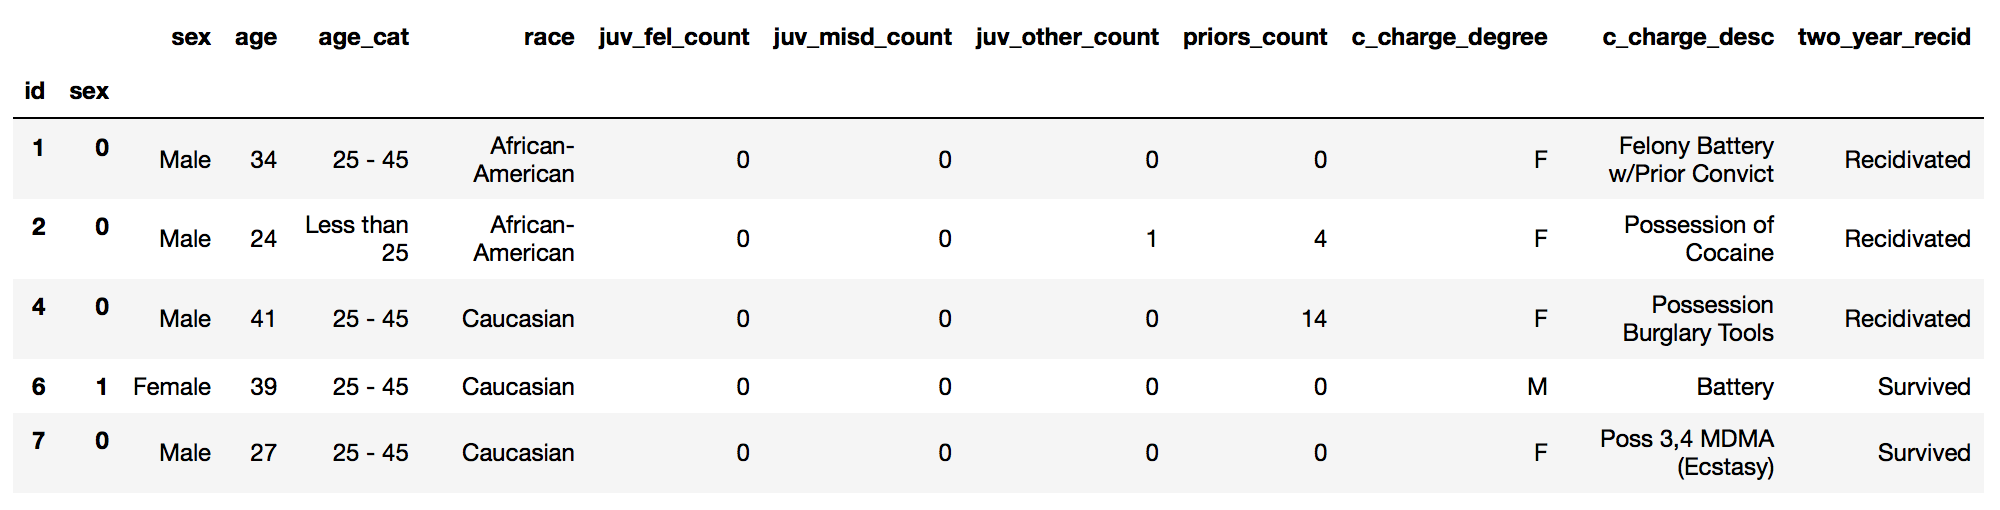
\includegraphics[width=1\linewidth]{../images/table_snippet} 

}

\caption{A snippet of the data set we will be using, containing information on a defendant's age, sex, race, criminal history, charge degree, charge description, and two-year recidivism outcome.}\label{fig:table snip}
\end{figure}

\begin{figure}

{\centering 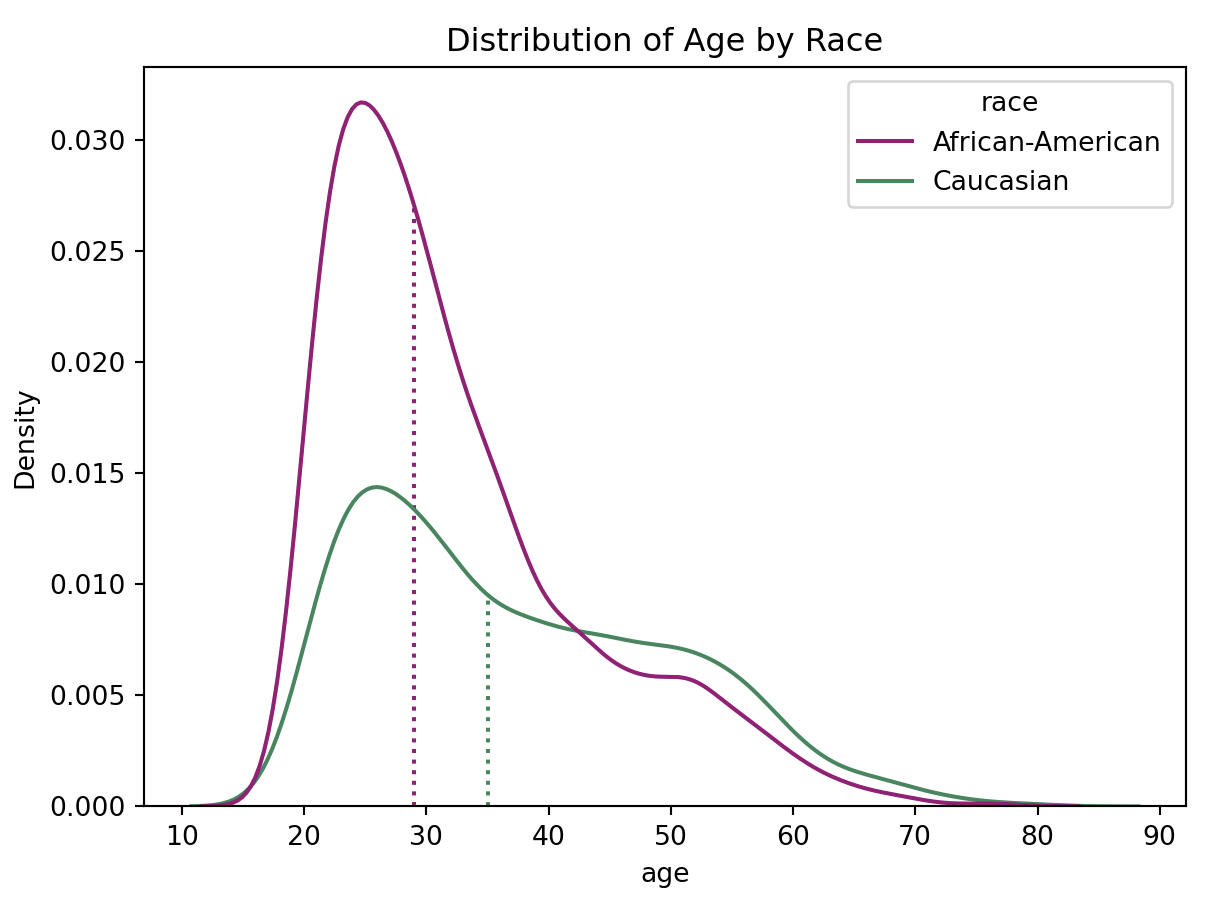
\includegraphics[width=1\linewidth]{../images/age_race_plot_new} 

}

\caption{The purple curve shows the distribution of the ages of Black defendants, and the green curve shows the distribution of the ages of white defendants. The probability of a defendant's age being between two points on the x-axis is the total shaded area of the curve under the two points. The purple dotted line represents the median age of Black defendants (29 years) and the green dotted line represents the median age of white defendants (35 years). For both groups, the majority of defendants are relatively young, but this is especially noticeable for Black defendants.}\label{fig:age plot}
\end{figure}

\begin{figure}

{\centering 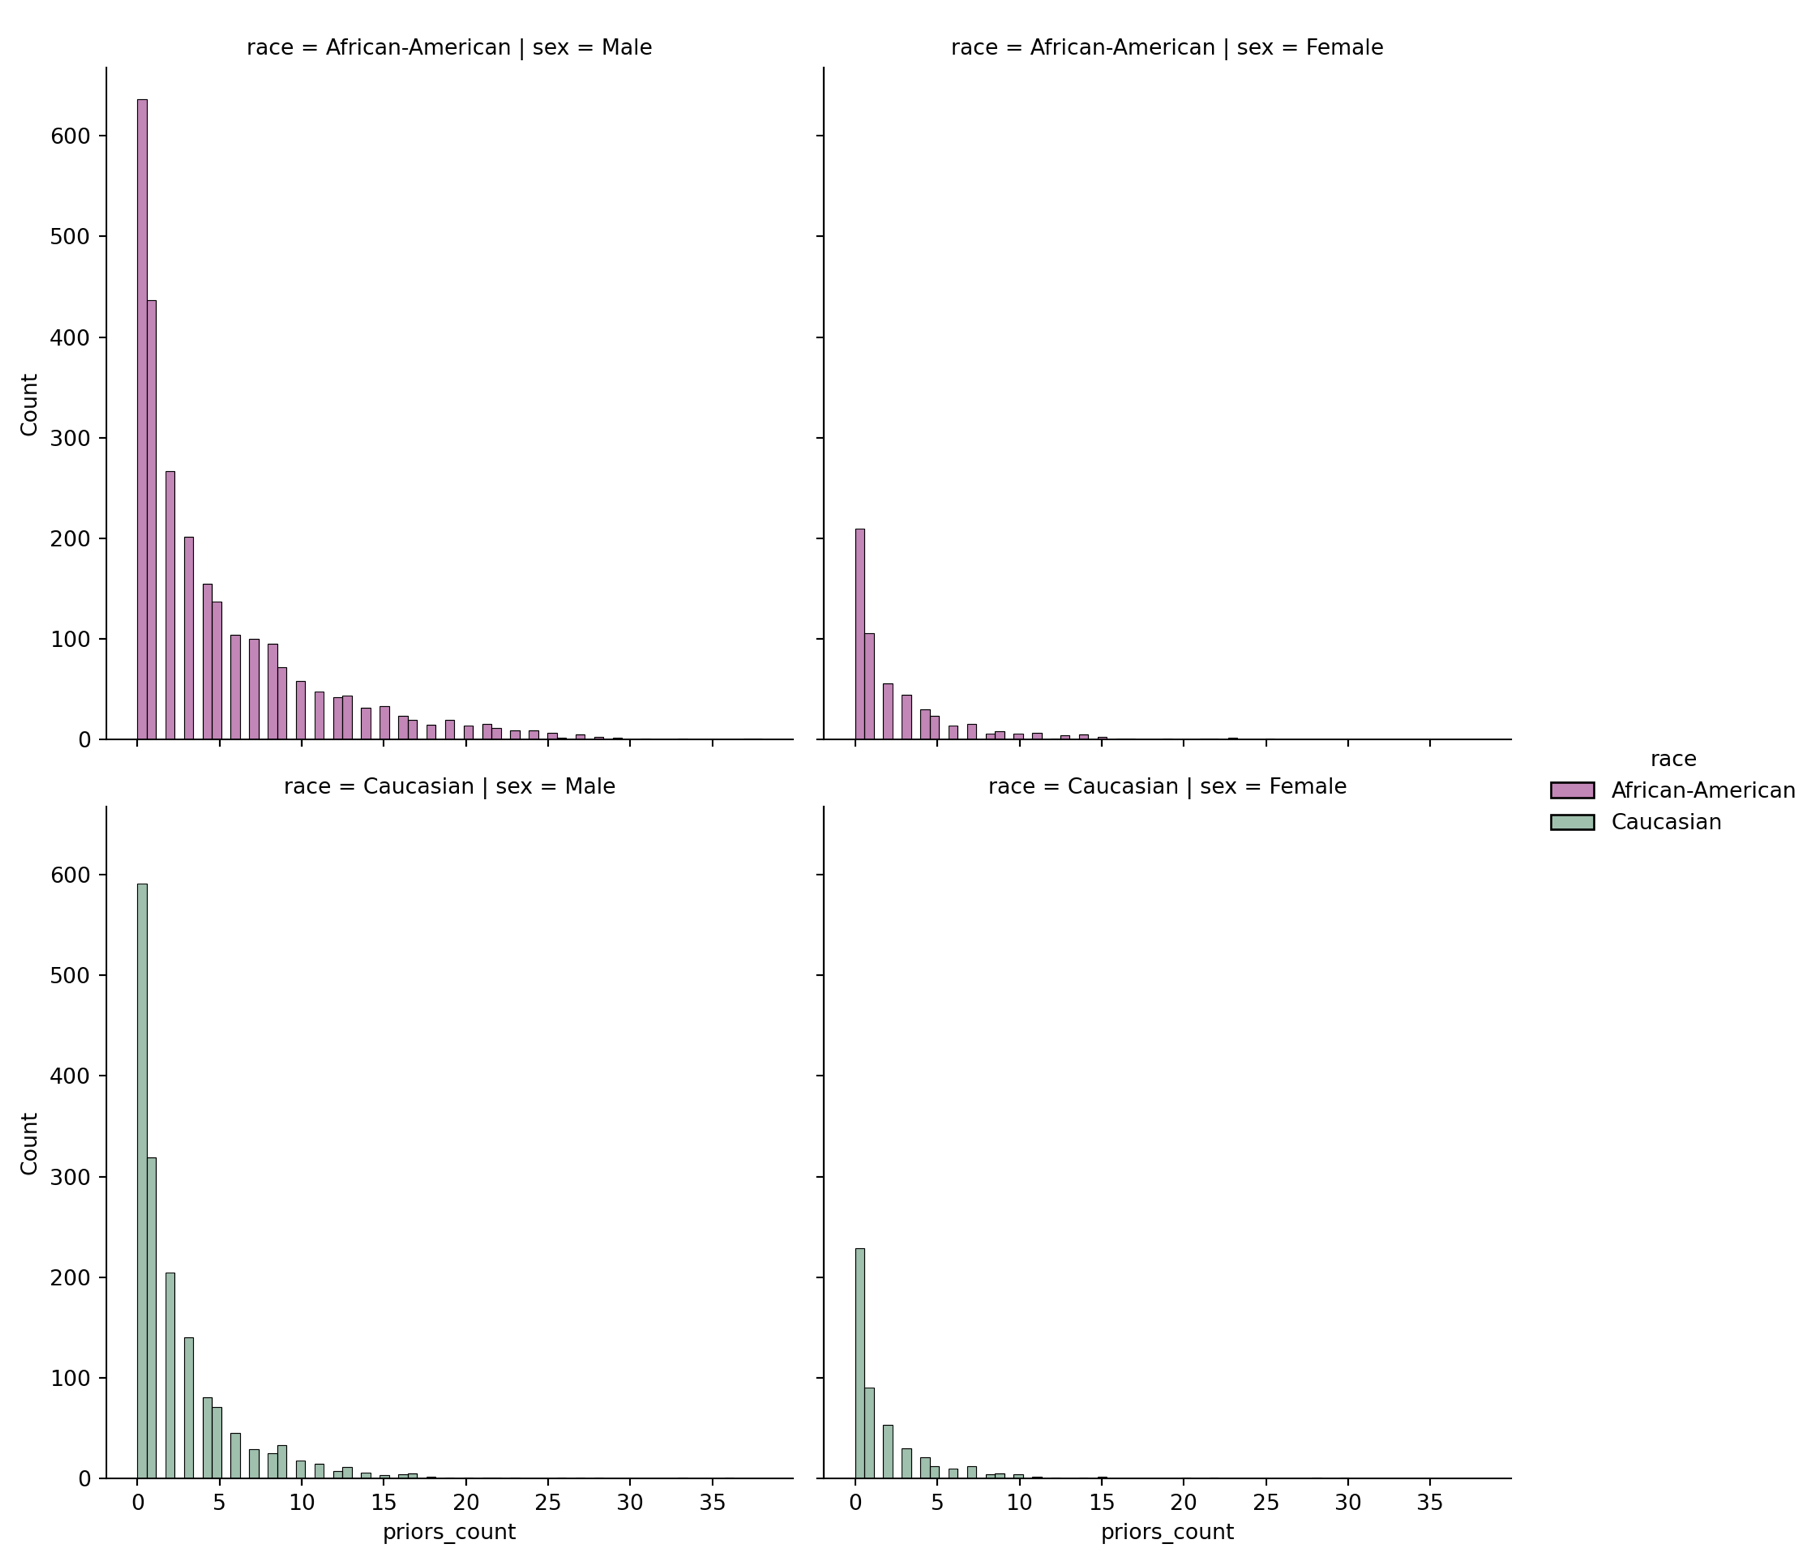
\includegraphics[width=1\linewidth]{../images/prior_charges_plot} 

}

\caption{Black defendants, particularly men, are more likely to have a greater count of prior charges than white defendants. Male defendants have a higher number of prior charges than do female defendants. Though we do not know for sure which information goes into the COMPAS algorithm, it is likely that a defendant with prior charges will be coded as a having a higher risk of recidivism. Thus, by looking at the racial discrepancies in prior charges we can already see potential bias in the algorithm.}\label{fig:prior plot}
\end{figure}

\begin{figure}

{\centering 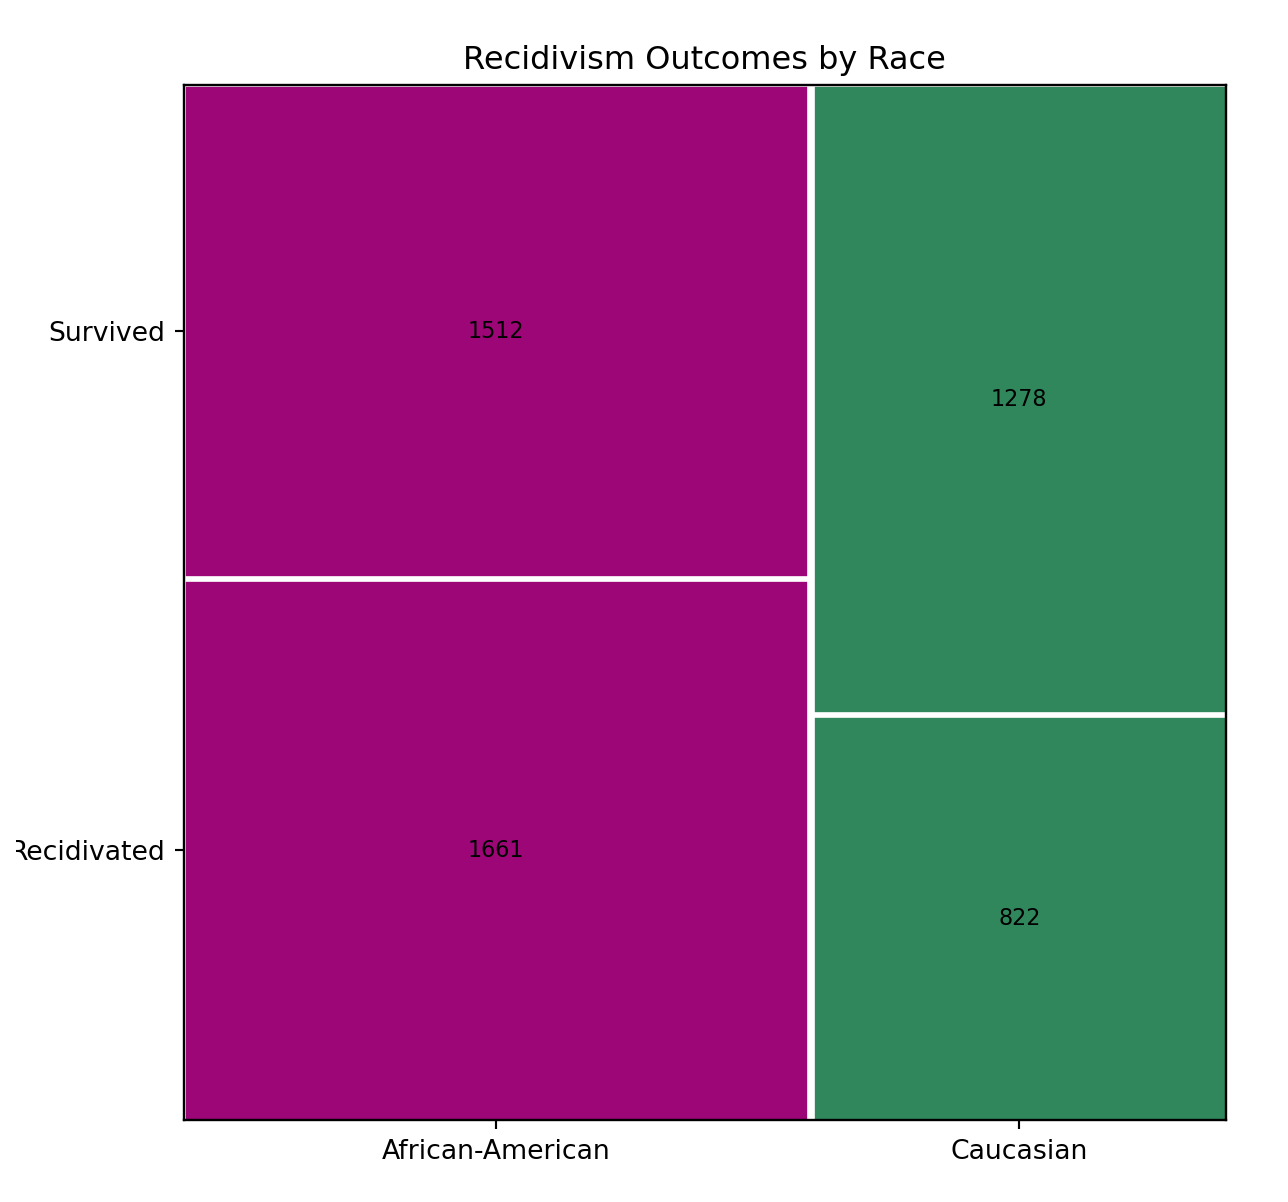
\includegraphics[width=1\linewidth]{../images/recidivism_mosaic} 

}

\caption{When we divide the data into Black and white defendants, we can see that Black defendants recidivate more than white defendants and Black defendants are more likely to recidivate than not recidivate. 39.14\% of white defendants did recidivate within two years compared to 52.35\% of Black defendants. We can also see that there are more Black defendants in the dataset overall.}\label{fig:recidivism mosaic}
\end{figure}

\begin{longtable}[]{@{}lrrr@{}}
\caption{Incidence of recidivism by race, illustrating how a much
greater proportion (\textgreater{} 50\%) of Black defendants recidivated
than their white counterparts. \label{tab:recid table}}\tabularnewline
\toprule
Two Year Recidivism by Race & Recidivated & Survived & Total \\
\midrule
\endfirsthead
\toprule
Two Year Recidivism by Race & Recidivated & Survived & Total \\
\midrule
\endhead
African American & 1661 & 1512 & 3173 \\
Caucasian & 822 & 1278 & 2100 \\
Total & 2483 & 2790 & 5273 \\
\bottomrule
\end{longtable}

\hypertarget{methods}{%
\section{Methods}\label{methods}}

AI Fairness 360 (AIF360) is an open-source Python toolkit that seeks
``to help facilitate the transition of fairness research algorithms to
use in an industrial setting and to provide a common framework for
fairness researchers to share and evaluate algorithms''
\citep{aif360-oct-2018}. It contains multiple data sets, including the
COMPAS data set that accompanied \citet{angwin2016machine}.

The AIF360 toolkit contains various group and individual fairness
metrics as well as pre-processing, in-processing, and post-processing
algorithms that we used to debias the COMPAS algorithm
\citep{aif360-oct-2018}. Fairness metrics are mathematical measures of
whether an algorithm treats members of different groups (such as racial
or gender groups) equally. An algorithm has no understanding of the
historical oppression of certain groups and how such bias is baked into
the data on which the algorithm is trained. Thus, fairness metrics
provide a method of evaluating an algorithm's level of bias towards or
against the unprivileged group versus the privileged group. We
researched the definitions and applications of different fairness
metrics \citep{ashokan2021fairness} to determine which metric would be
most appropriate for our project.

Fairness is subjective; one person might consider an algorithm fair if
groups are given the same treatment, while someone else might only
consider the algorithm fair if groups as a whole receive the same
outcomes. In our research we choose to use the definition of group
fairness as our definition for assessing fairness in the processing
approach. Group fairness metrics take into account the attributes of a
whole group as opposed to just one individual in the group, allowing us
to represent systemic issues. In general, group fairness metrics require
that the unprivileged group is treated similarly to the privileged
group, whereas individual fairness metrics require individuals to be
treated consistently \citep{kypraiou_what_2021}. Group and individual
metrics work in opposition of one another, meaning that when group
fairness improves, individual fairness gets worse
\citep{kypraiou_what_2021}. We chose the following four group fairness
metrics to evaluate our models.

\hypertarget{statistical-parity-difference}{%
\subsection{Statistical Parity
Difference}\label{statistical-parity-difference}}

This metric measures the difference between privileged and marginalized
groups' likelihood to get a particular outcome. The ideal value of this
metric is 0. Fairness for this metric is between -0.1 and 0.1. A
negative value means there is higher benefit for the privileged group
(in this case, white defendants).

\[P(\hat{Y}=1|D=Unprivileged) - P(\hat{Y}=1|D=Privileged)\]

\hypertarget{disparate-impact-ratio}{%
\subsection{Disparate Impact Ratio}\label{disparate-impact-ratio}}

This metric is the ratio of how often the favorable outcome occurs in
one group versus the other. In the case of recidivism, this is the ratio
of how many white defendants are predicted to not recidivate compared to
how many black defendants are predicted to not recidivate. A value of 1
means that the ratio is exactly 1:1. Less than 1 means the privileged
group (white defendants) benefits, while a value greater than 1 means
the unprivileged group (Black defendants) benefits. According to AIF360,
a ratio between 0.8 to 1.25 is considered fair \citep{Ronaghan2019AI}.

\[\frac{P(\hat{Y}=1|D=Unprivileged)}{P(\hat{Y}=1|D=Privileged)}\]

\hypertarget{equal-opportunity-difference}{%
\subsection{Equal Opportunity
Difference}\label{equal-opportunity-difference}}

The
\href{https://developers.google.com/machine-learning/glossary/fairness\#e}{equal
opportunity difference} metric is computed as the difference of true
positive rates between the unprivileged and the privileged groups. The
true positive rate is the ratio of true positives to the total number of
actual positives for a given group.

The ideal value is 0. A value less than 0 implies higher benefit for the
privileged group and a value greater than 0 implies higher benefit for
the unprivileged group. Fairness for this metric is between -0.1 and 0.1
\citep{aif360-oct-2018}.

This metric is best used when it is very important to catch positive
outcomes while false positives are not exceptionally problematic
\citep{Cortez2019How}. This is not the case for the COMPAS data set, as
false positives mean extra jail time for someone who will not actually
re-offend.

\[TPR_{D = Unprivileged} - TPR_{D = Privileged}\]

\hypertarget{average-odds-difference}{%
\subsection{Average Odds Difference}\label{average-odds-difference}}

This metric returns the average difference in false positive rate and
true positive rate for the privileged and unprivileged groups. A value
of 0 indicates equality of odds, and a value below 0 implies benefit for
the privileged group. Equality of odds is achieved in the case of
recidivism when the proportion of people who were predicted to
recidivate and did recidivate is equal (true positive rate) for both
Black and white defendants AND the proportion of people who were
predicted to recidivate and did not recidivate (false positive rate) is
equal for both Black and white defendants \citep{aif360-oct-2018}.

\[\frac{1}{2}\left[(FPR_{D = Unprivileged} - FPR_{D = Privileged}) + \underbrace{(TPR_{D = Unprivileged} - TPR_{D = Privileged})}_\textrm{Equal Opportunity Difference}\right]\]

For the next step of our experiment, we sought to determine where in the
data science pipeline we can mitigate the most bias, using
pre-processing, in-processing, and post-processing debiasing algorithms.
These are all based on using predictive models to figure out how we can
``fix'' the bias that is present.

\hypertarget{pre-processing}{%
\subsection{Pre-Processing}\label{pre-processing}}

Pre-processing refers to mitigating bias within the training data, and
it is the most flexible method because it has not yet trained a model
that may carry assumptions about the data. It is important to keep in
mind that pre-processing prevents assumptions in the modeling, but does
not account for the bias in data collection. Training data is where bias
is most likely to be introduced. We use the reweighing pre-processing
algorithm from AIF360 which assigns weights to the data. ``The advantage
of this approach is, instead of modifying the labels, it assigns
different weights to the examples based upon their categories of
protected attribute and outcome such that bias is removed from the
training dataset. The weights are based on frequency counts. However as
this technique is designed to work only with classifiers that can handle
row-level weights, this may limit your modeling options''
\citep{Ronaghan2019AI}. We used a logistic regression model for this
algorithm, as it is the easiest to interpret in the given context. After
running the fairness metrics using the pre-processing algorithm, we were
able to compare our results to the baseline metrics from the previous
section.

\hypertarget{in-processing}{%
\subsection{In-Processing}\label{in-processing}}

In-processing mitigates bias in classifiers while building a model. A
classifier ``is an algorithm that automatically orders or categorizes
data into one or more sets'' \citep{baxter2021AI}. The in-processing
technique we use is the prejudice remover algorithm, which accounts for
the fairness metric as part of the input and returns a classifier
optimized by that particular metric. In order to do this, we first
needed to convert our data frame into a data type called a
BinaryLabelDataset.

The prejudice remover is a method for reducing indirect prejudice (i.e.,
how COMPAS is racially biased because it uses proxy variables for race).
The prejudice remover implements two different regularizers, one to
avoid overfitting and one to enforce fair classification
\citep{kamishima2012fairness}. The prejudice remover regularizer works
by minimizing the prejudice index, a mathematical equation for
quantifying fairness defined by \citet{kamishima2012fairness}. This in
turn enforces a classifier's independence from sensitive information
(e.g., race). Similarly to pre-processing, we compared the results of
our in-processing methods with both the baseline and the pre-processing
model to gauge which method so far has the better group fairness.

\hypertarget{post-processing}{%
\subsection{Post-Processing}\label{post-processing}}

Our last approach, post-processing bias mitigation, is implemented after
training a model. Post-processing algorithms equalize the outcomes
(i.e., predicted recidivism values) to mitigate bias instead of
adjusting the classifier or the training data \citep{baxter2021AI}. We
use calibrated equalized odds, which ``optimizes over calibrated
classifier score outputs to find probabilities with which to change
output labels with an equalized odds objective''
\citep{aif360-oct-2018}. An equalized odds objective constrains
classification algorithms such that no error type (false-positive or
false-negative) disproportionately affects any population subgroup; both
groups, in our case both white and Black defendants, should have the
same false-positive and false-negative rates \citep{pleiss2017fairness}.
Through the calibrated equalized odds method, we want to decrease bias
while also maintaining calibration \citep{pleiss2017fairness}.
\href{https://medium.com/analytics-vidhya/calibration-in-machine-learning-e7972ac93555}{Calibration}
refers to improving a model so that the distribution of predicted
outcomes is similar to the distribution of observed probability in the
training data.

\hypertarget{results}{%
\section{Results}\label{results}}

With our baseline model, we ran the four different group fairness
metrics we chose and compared the results (pictured in Table
\ref{tab:baseline metrics table}).

The statistical parity difference is -0.14. This indicates that there is
a large difference between white and Black defendants regarding whether
or not they recidivate. The algorithm unfairly benefits white defendants
over Black defendants.

Disparate impact ratio is 0.47. The ratio of white defendants predicted
to not recidivate to Black defendants predicted to not recidivate is
0.47. A ratio between 0.8 and 1.25 is considered fair, therefore the
algorithm unfairly benefits white defendants.

Average odds difference is -0.44. The average difference in false
positive rates and true positive rates for white and Black defendants is
-0.44. Values less than zero are considered in favor of the privileged
group, so the algorithm unfairly benefits white defendants.

Equal opportunity difference is -0.41. The difference of true positive
rates between the Black and white groups is -0.41. A value less than 0
indicates a benefit to the privileged group, so the algorithm benefits
white defendants. The value is substantially less than -0.1, which
indicates that the algorithm is unfair.

All four group fairness metrics determine that the COMPAS algorithm
favors white defendants over Black defendants. Although the magnitudes
of the various fairness metrics are different, none of the metrics are
within their respective fairness thresholds. Our goal is to use
pre-processing, in-processing, and post-processing algorithms in the
AIF360 toolkit to see if we can make COMPAS fair at all.

Our confusion matrix for the baseline model indicates that the false
positive and false negative percentages are 16.68\% and 22.06\%, which
are the lowest values for this matrix. The highest value is the value of
true positives, at 35.41\%, showing that of the total number of
predictions, 35.41\% were correct predictions of recidivism.

\begin{longtable}[]{@{}llll@{}}
\caption{Results of Baseline Fairness Metric Analysis
\label{tab:baseline metrics table}}\tabularnewline
\toprule
Fairness Metric & Ideal Value & Baseline Value & Benefited Group \\
\midrule
\endfirsthead
\toprule
Fairness Metric & Ideal Value & Baseline Value & Benefited Group \\
\midrule
\endhead
Statistical Parity Difference & 0 & -0.14 & White Defendants \\
Disparate Impact Ratio & 1 & 0.47 & White Defendants \\
Average Odds Difference & 0 & -0.44 & White Defendants \\
Equal Opportunity Difference & 0 & -0.41 & White Defendants \\
\bottomrule
\end{longtable}

\hypertarget{pre-processing-approach-reweighing}{%
\subsection{Pre-Processing Approach:
Reweighing}\label{pre-processing-approach-reweighing}}

After running the reweighing algorithm, our fairness metrics are -0.015
for statistical parity difference, 0.015 for equal opportunity
difference, 0.014 for average odds difference, and 0.98 for disparate
impact ratio. All of these values now fall within the margins of
fairness (see reweighing metrics plot). These values make sense because
the reweighing algorithm chooses different weights depending on whether
an attribute is protected. This does an effective job of eliminating the
bias, shown by each of the values in the graph being within the ``fair''
range of the particular fairness metric. Overall, these fairness metrics
show that the reweighing algorithm improves the bias in the COMPAS
algorithm.

The highest percentage in this confusion matrix is for the percentage of
true negatives, defendants who were predicted to not recidivate and
actually did not, at 36.24\%, 0.83\% higher than the true negatives in
the baseline model. This means that the reweighing model marginally
improved the baseline model accuracy in predicting people who did not
recidivate. However, the percentage of true positives, or those who were
predicted to recidivate and did recidivate, is 24.72\%, 1.13\% lower
than that of the baseline model. This means that the reweighing model
slightly lowered the accuracy of the baseline model in predicting people
who did recidivate. As a result, the overall reweighing model accuracy
remains about the same as the baseline model accuracy. The false
negative and false positive percentages, or the predictions that proved
to be incorrect, are 23.20\% and 15.85\%, respectively. The re-weighing
model increased the number of false negatives by 1.14\% and decreased
the number of false positives by 0.83\%. We are most concerned about the
false positives, which indicate defendants who are predicted to
recidivate and do not actually recidivate. While there is a slight
improvement in the percent of false positives, it is still relatively
high at 15.85\%, indicating that we should further precede with
additional bias mitigation techniques.

\hypertarget{in-processing-approach-prejudice-remover}{%
\subsection{In-Processing Approach: Prejudice
Remover}\label{in-processing-approach-prejudice-remover}}

Our fairness metrics after running the prejudice remover are: 0.367 for
statistical parity difference, 0.321 for equal opportunity difference,
0.344 for average odds difference, and 3.3 for disparate impact ratio.
Like the model performance metrics suggested, the prejudice remover
approach resulted in an increased benefit for Black defendants. As the
orange bars on these plots show, the values of the fairness metrics have
reversed from their baseline values. Now all four metrics suggest an
unfair advantage for Black defendants. Thus, this approach removed the
model's prejudice against Black people, but it did not result in a
``fair'' model.

The highest percentage in this confusion matrix is for false positives,
defendants who the model predicted to recidivate and actually did not,
at 37.76\%. This false positive percentage concerns us because we do not
want defendants who do not recidivate to have unfairly long sentences
due to their (incorrectly) predicted recidivism. The number of true
positives, defendants who the model predicted to recidivate and actually
recidivated, is lower at 23.88\%. The percentage of false negatives is
lower, whereas the true negative is low at 14.33\%. This indicates that
the model does not do a good job in predicting the defendants who don't
recidivate. It is very likely that it will incorrectly predict that
someone will recidivate.

After the prejudice remover, the accuracy of the model is fairly similar
across the board of races, but the model's accuracy is only 38.21\%,
which is much lower than the baseline and reweighing models. This
accuracy score means that the model makes accurate predictions only 38\%
of the time.

\hypertarget{post-processing-approach-calibrated-equalized-odds}{%
\subsection{Post-Processing Approach: Calibrated Equalized
Odds}\label{post-processing-approach-calibrated-equalized-odds}}

After running the calibrated equalized odds algorithm, our fairness
metrics are: 0.134 for statistical parity difference, 0.088 for equal
opportunity difference, 0.146 for average odds difference, and 1.155 for
disparate impact ratio. As we can see from the orange bars, the
calibrated equalized odds approach results in all four metrics now
suggesting a benefit for the originally unprivileged group, Black
defendants. Though the values for statistical parity difference and
average odds difference are slightly above the range of what is
considered fair, the margin is much smaller than the original margin
between the value and the range of fairness (as indicated by the blue
bars). Thus, the calibrated equalized odds approach successfully
counteracts the bias against Black defendants and results in a mostly
fair model.

The highest percentage in this confusion matrix is for true negatives,
defendants who the model predicted to not recidivate and actually did
not, at 50.04\%. The number of true positives, defendants who the model
predicted to recidivate and actually recidivated, is much lower at
3.11\%. The percentage of false negatives is somewhat high for this
baseline model, whereas the amount of false positives is very low at
2.05\%. This indicates that the model does a good job in predicting the
defendants who don't recidivate. It is very unlikely that it will
incorrectly predict that someone will recidivate. Though the accuracy
score for the model is 0.53, lower than the baseline, this model is much
better at identifying true negatives.

\hypertarget{conclusion}{%
\section{Conclusion}\label{conclusion}}

\hypertarget{limitations}{%
\subsection{Limitations}\label{limitations}}

Our project tries to mitigate bias within existing data, rather than
within the methods used to collect this data. The data are collected
using a risk assessment survey, where defendants are asked a series of
questions (see introduction) which are supposedly used to determine
whether someone will recidivate or not. Many of these questions involve
proxy variables for race. The creation and facilitation of this survey
can therefore be assessed for bias mitigation as the methods used may
potentially privilege some groups over others. As a result, the bias
exists even before values are collected, limiting the debiasing work
able to be done on the output values.

Furthermore, AIF360 processed the data we used in this project the same
way ProPublica processed their data. AIF360 simplifies the original
defendant data and their COMPAS scores to make the data easier to
analyze. However, this initial processing may lose some details captured
in the original raw data. As we have noted throughout this paper, bias
can be introduced in any step of the data science pipeline and AIF360's
initial data processing step is no exception.

AIF360 contains an array of processing methods that have been written by
various scholars of fairness \citep{aif360-oct-2018}. These methods are
each distinct and apply a different technique to mitigate bias. Our
results only contain three processing methods, one for each step in
processing. This choice was based on time constraints as well as our
working environment. For example, the code for most of the other
in-processing methods would not run for us. In-processing on its own
works to debias an algorithm, not the input or output values, so some of
those methods may not work on certain algorithms. We had similar
challenges with pre and post-processing, where the methods were
challenging to run and would require more time to be spent debugging in
order to make them work. Had we used alternative processing methods, our
results would be quite different, as the method changes apply a
different mathematical technique to the input.

\hypertarget{future-work}{%
\subsection{Future Work}\label{future-work}}

In this project, we have only focused on a few select fairness metrics
and a few debiasing algorithms. We looked at group fairness metrics
because we specifically wanted to mitigate systemic racial bias in the
COMPAS algorithm, but other researchers could compare how well debiasing
algorithms work using individual fairness metrics. Future work could
also include conducting more tests using other debiasing algorithms to
see if the COMPAS algorithm could be made more fair. One significant
limitation of our work is that some of the in-processing algorithms
provided in the AIF360 toolkit were difficult to integrate into our code
and we were unable to run many of them. The processing methods we chose,
though effective, were based on our work environments, and there are
other existing algorithms that attempt to mitigate bias.

We only looked at defendants labeled as Caucasian and African-American
in our dataset, which diminishes the generalizability and nuance of our
results. Comparing how COMPAS assesses defendants of other races would
be an incredibly relevant extension of our existing work. Furthermore,
\citet{larson2016we} also found that age was the most predictive factor
of a higher risk score: ``Defendants younger than 25 years old were 2.5
times as likely to get a higher score than middle aged offenders, even
when controlling for prior crimes, future criminality, race and gender''
\citep{larson2016we}. In addition, female defendants were more likely to
receive a higher recidivism risk score than male defendants when
controlling for the aforementioned factors \citep{larson2016we}. Thus,
some extensions of our work could include attempting to remove age and
gender bias and determining the most effective processing algorithms to
do so.

The dataset we are working with only contains defendants' criminal
history records from Broward County, Florida. Many other states,
including New York and Massachusetts, use COMPAS to calculate recidivism
scores, and a further study could apply this paper's methods to the data
coming out of other states. By conducting experiments on multiple states
the baseline model would be trained on a larger and more diverse set of
data, which could improve its accuracy. In addition, by adding more
geographically diverse data to our set we can start to create more
generalizable conclusions about our results. However, future researchers
must keep in mind the real-life consequences of recidivism risk
algorithms like COMPAS and how research on methods of debiasing
algorithms could potentially be utilized to justify the continued use of
biased algorithms.

\hypertarget{final-thoughts}{%
\subsection{Final Thoughts}\label{final-thoughts}}

Through our methods, we concluded that the pre-processing and
post-processing methods mitigate bias and increase fairness most
successfully. The in-processing technique was effective at mitigating
bias, but did not result in a mathematically fair model. However, these
techniques only treat the symptoms of racial bias in the justice system,
as opposed to addressing the root cause, systemic racism. We need to
question why these flawed algorithms exist and why they can be used to
determine someone's fate in the justice system. While we may have
methods for reducing bias algorithms such as COMPAS, the focus should be
on addressing the over-policing and over-criminalization of Black
communities that result in biased data and algorithms.

\hypertarget{ethical-statement}{%
\subsection{Ethical Statement}\label{ethical-statement}}

Throughout this project, we endeavored to debias an incredibly powerful
algorithm that can change the course of someone's life. However, we want
to recognize that debiasing methods are not the most effective or
beneficial way to uproot bias within the American justice system. The
problems within the justice system are much more complex than an
algorithm and are rooted in the United States's history of racism. In
addition, algorithmic bias is much more complex than the algorithm
itself; algorithmic bias comes from the people who produce the
algorithm. We all have our own beliefs, biases, and situated knowledge
that impact and subsequently limit everything we create.

\hypertarget{acknowledgements}{%
\section{Acknowledgements}\label{acknowledgements}}

We would like to thank our sponsor organization Women At The Table and
Professor Ben Baumer for introducing us to this incredibly meaningful
work, supporting us, and answering the many questions we had throughout
this semester-long project. We would specifically like to thank Sofia
Kypraiou for her mentorship and patience throughout this process.

% %%%%%%%%%%%%%%%%%%%%%%%%%%%%%%%%%%%%%%%%%%
% %% optional
% \supplementary{The following are available online at www.mdpi.com/link, Figure S1: title, Table S1: title, Video S1: title.}
%
% % Only for the journal Methods and Protocols:
% % If you wish to submit a video article, please do so with any other supplementary material.
% % \supplementary{The following are available at www.mdpi.com/link: Figure S1: title, Table S1: title, Video S1: title. A supporting video article is available at doi: link.}

\vspace{6pt}

%%%%%%%%%%%%%%%%%%%%%%%%%%%%%%%%%%%%%%%%%%

%%%%%%%%%%%%%%%%%%%%%%%%%%%%%%%%%%%%%%%%%%

%%%%%%%%%%%%%%%%%%%%%%%%%%%%%%%%%%%%%%%%%%

%%%%%%%%%%%%%%%%%%%%%%%%%%%%%%%%%%%%%%%%%%
%% optional


%%%%%%%%%%%%%%%%%%%%%%%%%%%%%%%%%%%%%%%%%%
% Citations and References in Supplementary files are permitted provided that they also appear in the reference list here.

%=====================================
% References, variant A: internal bibliography
%=====================================
%\reftitle{References}
%\begin{thebibliography}{999}
% Reference 1
%\bibitem[Author1(year)]{ref-journal}
%Author1, T. The title of the cited article. {\em Journal Abbreviation} {\bf 2008}, {\em 10}, 142--149.
% Reference 2
%\bibitem[Author2(year)]{ref-book}
%Author2, L. The title of the cited contribution. In {\em The Book Title}; Editor1, F., Editor2, A., Eds.; Publishing House: City, Country, 2007; pp. 32--58.
%\end{thebibliography}

% The following MDPI journals use author-date citation: Arts, Econometrics, Economies, Genealogy, Humanities, IJFS, JRFM, Laws, Religions, Risks, Social Sciences. For those journals, please follow the formatting guidelines on http://www.mdpi.com/authors/references
% To cite two works by the same author: \citeauthor{ref-journal-1a} (\citeyear{ref-journal-1a}, \citeyear{ref-journal-1b}). This produces: Whittaker (1967, 1975)
% To cite two works by the same author with specific pages: \citeauthor{ref-journal-3a} (\citeyear{ref-journal-3a}, p. 328; \citeyear{ref-journal-3b}, p.475). This produces: Wong (1999, p. 328; 2000, p. 475)

%=====================================
% References, variant B: external bibliography
%=====================================
\reftitle{References}
\externalbibliography{yes}
\bibliography{mybibfile.bib}

%%%%%%%%%%%%%%%%%%%%%%%%%%%%%%%%%%%%%%%%%%
%% optional

%% for journal Sci
%\reviewreports{\\
%Reviewer 1 comments and authors’ response\\
%Reviewer 2 comments and authors’ response\\
%Reviewer 3 comments and authors’ response
%}

%%%%%%%%%%%%%%%%%%%%%%%%%%%%%%%%%%%%%%%%%%


\end{document}
